\documentclass[tikz]{standalone}
\usetikzlibrary{patterns}
\usetikzlibrary{shapes,arrows}
\usetikzlibrary{decorations.pathreplacing, positioning}
\definecolor{greengreen}{rgb}{0.0, 0.42, 0.24}
\definecolor{calpolypomonagreen}{rgb}{0.12, 0.3, 0.17}
\definecolor{forestgreen}{rgb}{0.13, 0.55, 0.13}

\begin{document}
\noindent
  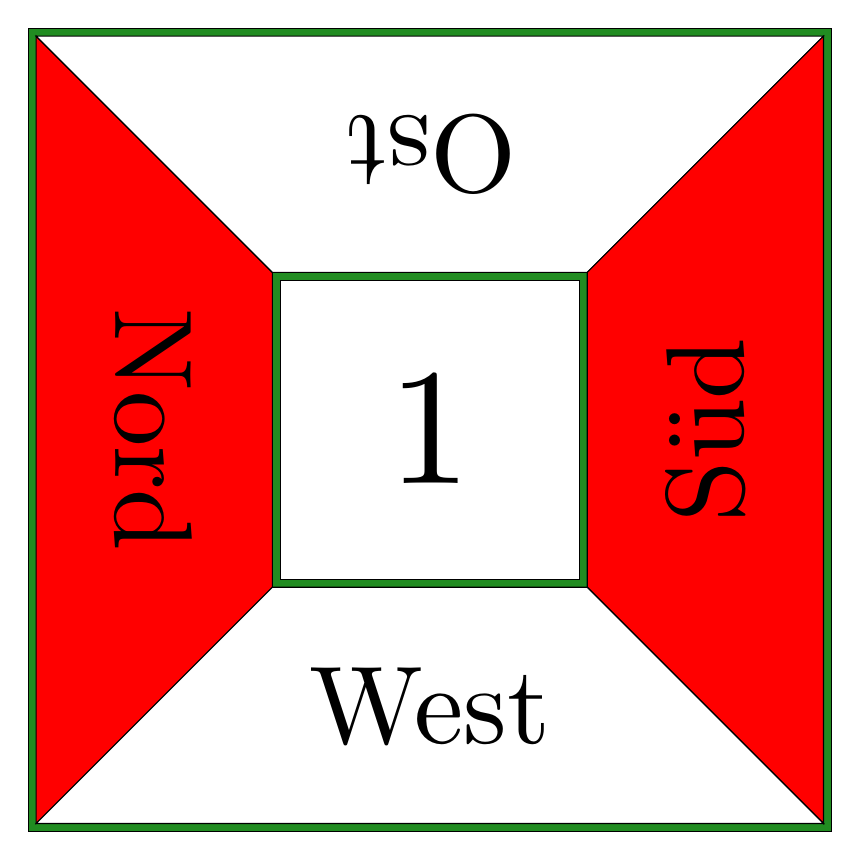
\begin{tikzpicture}

    \draw[fill=forestgreen] (-0.1,-0.1) -- (-0.1,10.1) -- (10.1, 10.1) -- (10.1, -0.1) -- cycle;
    \draw[fill=white] (0,0) -- (0,10) -- (10, 10) -- (10, 0) -- cycle;
    \draw[fill=forestgreen] (3, 3) -- (3,7) -- (7, 7) -- (7, 3) -- cycle;
    \draw[fill=white] (3.1, 3.1) -- (3.1,6.9) -- (6.9, 6.9) -- (6.9, 3.1) -- cycle;




    \draw[fill=red] (0,0) -- (0,10) -- (3, 7) -- (3, 3) -- cycle;
    \draw[fill=white] (0,10) -- (10,10) -- (7, 7) -- (3, 7) -- cycle;
    \draw[fill=red] (10,10) -- (10,0) -- (7, 3) -- (7, 7) -- cycle;
    \draw[fill=white] (0,0) -- (3,3) -- (7, 3) -- (10, 0) -- cycle;

    \node[very thick, rotate=270, scale=4] at (1.5,5) {Nord};
    \node[very thick, rotate=180, scale=4] at (5,8.5) {Ost};
    \node[very thick, rotate=90, scale=4] at (8.5, 5) {Süd};
    \node[very thick, rotate=0, scale=4] at (5, 1.5) {West};

    \node[very thick, rotate=0, scale=6] at (5, 5) {1};

  \end{tikzpicture}%
\end{document}
